\section{Gestion de projet}

\subsection{Phase de développement}

Le diagramme de Gantt ci-dessous (Figure 7) montre comment nous avons planifié 
notre projet [Posturo]. Il est organisé sur une durée de six semaines. 
Les semaines et les tâches de chacune d'elles sont divisées en plusieurs sections. 
Un ou plusieurs membres de l'équipe (Hippolyte, Inès et/ou Anaelle) sont chargés 
de chaque tâche, avec des durées adaptées en fonction de leur complexité et de 
leur importance. Par exemple, pour garantir leur qualité, des tâches essentielles 
telles que la conception de l'interface utilisateur ou l'intégration de graphiques 
demandent davantage de temps, tandis que des étapes préparatoires telles que la 
traduction des formules ou la création de la base de données sont planifiées sur 
des périodes plus courtes car moins complexes.

Les première semaines sont consacrées à poser les bases de notre logiciel, 
tandis que les semaines suivantes portent sur le développement et l'intégration 
des fonctionnalités avancées. Avant la livraison finale, les deux dernières 
semaines sont consacrées aux tests, à la préparation des présentations et à la 
vérification de nos modèles.

\begin{figure}[H]
    \centering
      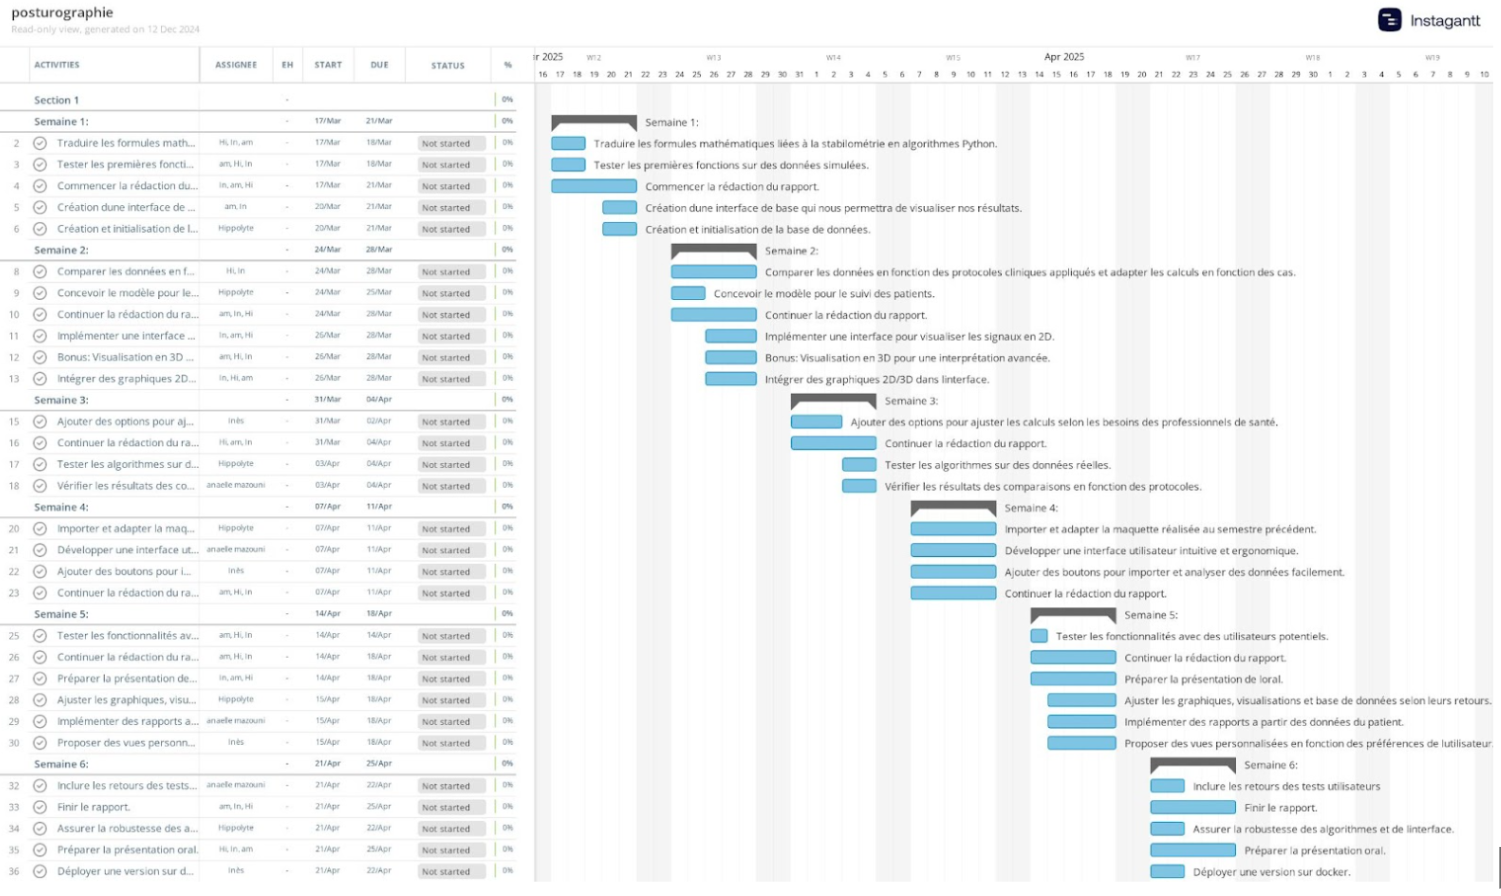
\includegraphics[height=10cm]{images/Gantt.png}
      \caption{diagramme de gantt réalisé sur instagantt}\label{fig:Gantt}
\end{figure}

\subsection{Outils utilisés}

Pour le premier semestre, nous avons utilisé Google Drive pour stocker les 
différentes versions de notre rapport et organiser des réunions hebdomadaires 
avec notre référente de projet. A fin d'assurer un suivi optimal pour le second semestre , des outils tels que le diagramme de Gantt, 
Trello et des réunions seront utilisés. Trello facilitera l'identification des tâches principales, l'ajout de 
sous-tâches non encore identifiées et la gestion quotidienne du travail. 
De son côté, le diagramme de Gantt propose une vision globale du projet, ce qui 
permet de prendre du recul sur l'avancement global et de repérer d'éventuels 
retards. L'équipe prévoit de tenir des réunions régulières afin de discuter des 
progrès réalisés et de rédiger un rapport hebdomadaire pour évaluer le progrès et 
résoudre les problèmes rencontrés. Les réunions seront plus informelles étant 
donné que nous ne sommes que trois dans ce projet, mais la communication 
quotidienne permettra de partager les avancées, les idées et les éventuels 
obstacles à surmonter, assurant ainsi une progression constante et efficace. 
Tous ces outils faciliteront la planification, le suivi des tâches et la 
résolution rapide des blocages.
